\lfoot{Autor: Raphael Simsek}
\subsubsection{OBD II}
\label{subsec:obd2}

\textbf{Defintion\nextline}
Die OBD-II Schnittstelle ist eine normierte, standardisierte Schnittstelle, welche, mittels passendem Auslesegerät, Zugriff auf die Daten des Motormanagements verschafft. Diese Schnittstelle hat unterschiedliche Versionen, welche auf die verschiedenen Kontinente aufgeschlüsselt wurden. 

\textbf{Standardisierung\nextline}
Es gibt also OBD II, welches ursprünglich eine Schnittstelle der vereinigten Staaten war, weshalb der Standard auch in Nordamerika seit 1996 verbaut wurde. Zusätzlich gibt es EOBD, womit die europäische Umsetzung des OBD II Standards beschrieben wird.\cite{SIMR.CH2-CAN-Bus.EUP-D98/69/EC} Der wesentliche Unterschied ist dabei die Standardisierung, welche zwar technisch zwischen SAE J1962 und ISO/DIS 15031 gleich ist, aber trotzdem unterschiedlich benannt wurde. \cite{SIMR.CH2-CAN-Bus.SAEJ1962} Ferner gab es eine australische \cite{SIMR.CH2-CAN-Bus.AU-MVSA1989} und eine japanische Version der Standardisierung.

\textbf{Charakterisierung\nextline}
Außerdem gibt es einen, ebenfalls in der Standardisierung festgelegten OBD II A und B Konnektor. Der A Konnektor ist für alle Fahrzeuge mit 12 V Bordspannung und hat die Form eines D mit einer Nut in der Mitte, um die Pins zu behausen. Der B Konnektor verwendet ebenfalls die Form eines D's, allerdings ist dieser Konnektor für Fahrzeuge mit 24V Bordspannung, welche häufig Lastkraftfahrzeuge sind. Bei diesem Konnektor ist die Nut in der Mitte unterbrochen, um es unmöglich zu machen einen männlichen Konnektor des A-Typs einzustecken. Dieser Konnektor könnte  nämlich aufgrund von Überspannung defekt werden. Es ist also der B Konnektor sowohl mit A und B kompatibel, allerdings ist der A Konnektor nur mit seinesgleichen verwendbar.

\begin{figure}[!htb]\centering
   \begin{minipage}{0.49\textwidth}
     \frame{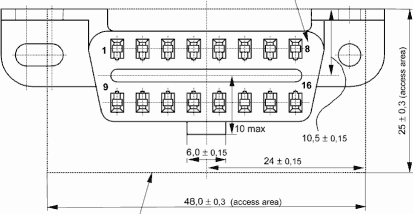
\includegraphics[width=\linewidth]{images/j1962f_type_a}}
     \caption{Typ A, OBD II Konnektor \cite{SIMR.CH2-CAN-Bus.OBDIITypeA}}\label{Fig:Data1}
   \end{minipage}
   \begin {minipage}{0.49\textwidth}
     \frame{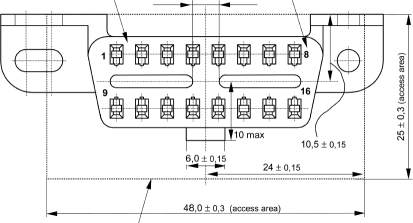
\includegraphics[width=\linewidth]{images/j1962f_type_b}}
     \caption{Typ B, OBD II Konnektor \cite{SIMR.CH2-CAN-Bus.OBDIITypeB}}\label{Fig:Data2}
   \end{minipage}
\end{figure}


\textbf{Positionierung / Lokalisierung\nextline}
Die OBD II Schnittstelle muss bei allen PKW mit Benzinmotor ab 2001 und bei allen PKW mit Dieselmotor ab 2004 im Sichtfeld des Fahrers verbaut sein. Aus diesem Grund wird die OBD II Schnittstelle von gängigen Automobilherstellern oft fahrerseitig im Bereich der Pedale, im Bereich der Mittelkonsole oder links neben dem Lenkrad montiert. Vor allem Fahrzeuge des VW-Konzerns integrieren Ihre OBD-II Schnittstelle auch im Sicherungskasten. Um besser zu veranschaulichen wo die OBD II Schnittstelle zumeist zu finden ist, wurde untersucht wo sich diese bei den verkaufsstärksten Produkten der verschiedenen Fahrzeugkategorien befindet.

\textbf{Kompaktklasse: Volkswagen Golf}
Exemplarisch können Sie hier die Lokalisierung der OBD II Schnittstelle an einem Golf VI erkennen. Diese Schnittstelle ist hier unterhalb einer ohne Werkzeug entfernbaren Abdeckung versteckt. Wie auf dem Foto erkennbar ist die Schnittstelle hier im Fußraum der Fahrerseite, links der Pedale platziert.

\begin{figure}[!htb]\centering
	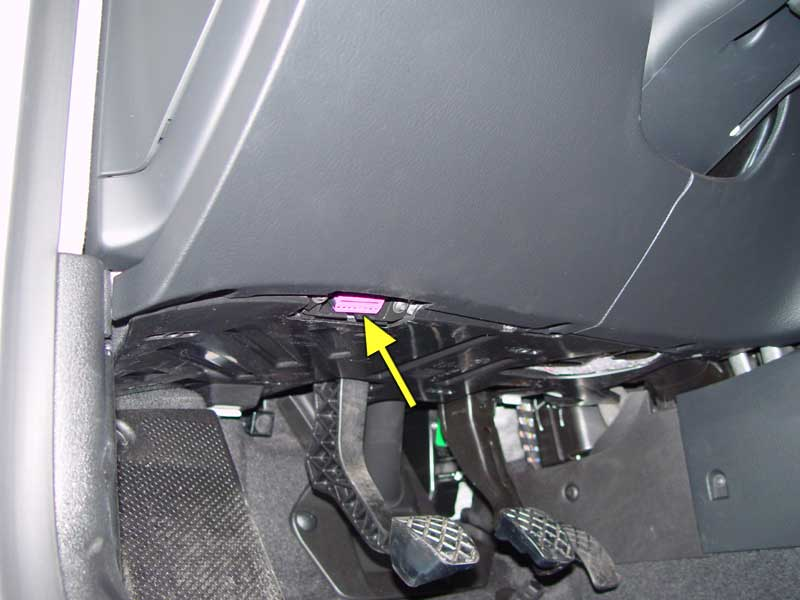
\includegraphics[width=0.5\textwidth]{images/golfobd}
	\caption{OBD II Konnektor bei einem Golf VI \cite{SIMR.CH2-CAN-Bus.GolfOBD}}\label{Fig:Data3}
\end{figure}

\textbf{Kleinwagen: Volkswagen Polo}
Erwartungsgemäß befindet sich der OBD Konnektor bei einem Fahrzeug des selben Herstellers an einer sehr ähnlichen Position, im Fußraum links der Pedale.

\begin{figure}[!htb]\centering
	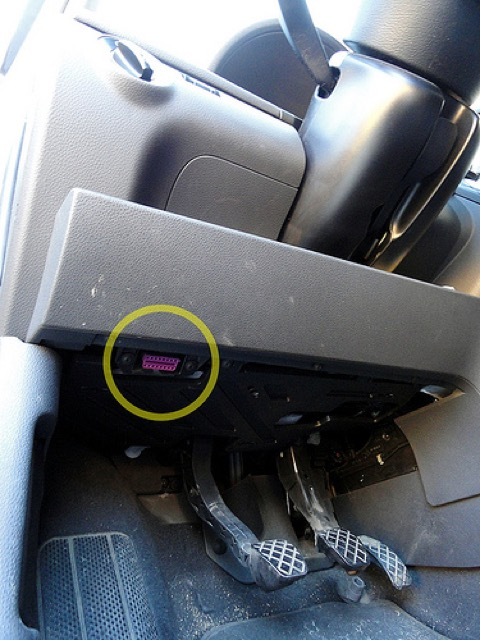
\includegraphics[width=0.25\textwidth]{images/poloobd}
	\caption{OBD II Konnektor bei einem Polo IV (Typ 9N3) \cite{SIMR.CH2-CAN-Bus.PoloOBD}}\label{Fig:Data3}
\end{figure}

\textbf{Mittelklasse: BMW 3er}
Bei einem BMW 3er E90 ist der OBD Konnektor auf der linken Fußraumverkleidung der Fahrerseite zu finden. Er wurde unter einer kleinen Abdeckung, welche mit \"OBD\" beschriftet ist, verdeckt. Die OBD Schnittstelle ist hier vertikal angeordnet, wie sie auf dem angeführten Bild sehen können.

\begin{figure}[!htb]\centering
	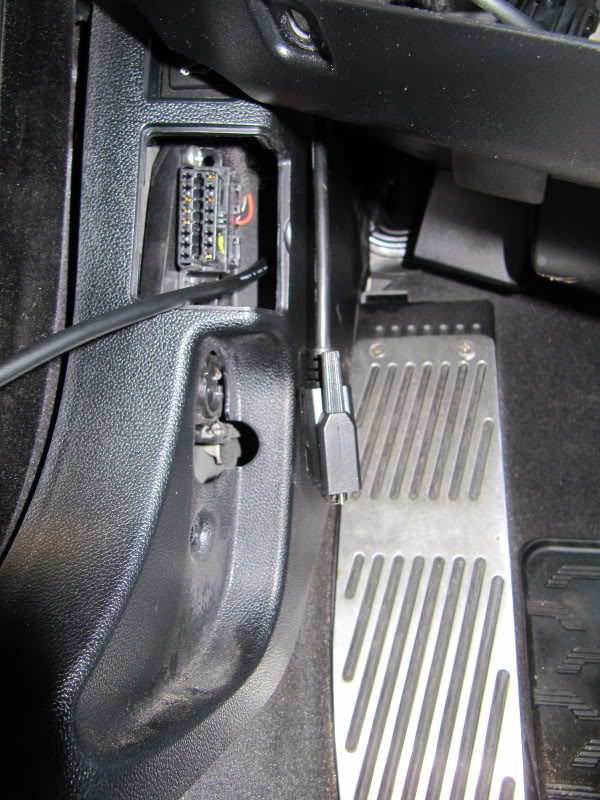
\includegraphics[width=0.6\textwidth]{images/3erobd}
	\caption{OBD II Konnektor bei einem BMW 3er E90 \cite{SIMR.CH2-CAN-Bus.3erOBD}}\label{Fig:Data3}
\end{figure}

\textbf{Auslesen und Verarbeiten\nextline}
Die OBD Schnittstelle muss natürlich, für eine weitere Verwendung,  ausgelesen werden. Dies ist bei einer derart seriellen Schnittstelle für einen Leihen schnell zu einer Herausforderung werden. Dabei kommen viele Hilfestellungen im Internet zur Hilfe. Jede Mode 1 PID X0 ist eine Überprüfungs-PID, die die unterstützten PID's Bitweise codiert auflistet. Im folgenden wird beschrieben wie man diese Bitweise codierten supported-PID's ausließt und das Ergebnis verarbeitet.

\begin{enumerate}
	\item Verbindung aufbauen
	\begin{enumerate}
		\item Verbindung mit Bluetooth OBD-II ELM327 Chip aufbauen
		\item Verbindung zum seriellen COM-Port aufbauen 
	\end{enumerate}
	\item 0100 abfragen
	\item Zurückgegebene 4 Byte von Hexadezimal zu Binär umrechnen
	\item In eine Tabelle einfügen und überprüfen welche PID's unterstützt sind
\end{enumerate}

Man ließt zuerst den Code 0100 aus, nachdem man sich mit dem Bluetooth Dongle verbunden hat und eine Verbindung mit dem seriellen COM-Port, welchen man im Geräte Manager finden kann, mittels Putty oder iTerm aufgebaut wurde.
Als Antwort auf seine Anfrage bekommt man 4 Byte Daten geliefert, die so \textit{BE1FA813} aussehen können. Danach muss man diese Daten, mit einem Umrechner, von Hexadezimal zu Binär umrechnen. Wenn diese Abrechnung abgeschlossen ist bekommt man eine 32-stellige Zahlenkette, jeweils zwischen 0 und 1. 
Diese kann man in folgende Tabelle einfügen und so erkennen welche PID's unterstützt werden.

\begin{table}[!htb]
\centering
\begin{tabular}{|l|c|c|c|c|c|c|c|c|c|c|c|c|c|c|c|c|}
\hline
Hexadecimal & \multicolumn{4}{c|}{B} & \multicolumn{4}{c|}{E} & \multicolumn{4}{c|}{1} & \multicolumn{4}{c|}{F} \\ \hline
Binary & 1 & 0 & 1 & 1 & 1 & 1 & 1 & 0 & 0 & 0 & 0 & 1 & 1 & 1 & 1 & 1 \\ \hline
Supported? & \cellcolor[HTML]{9AFF99}Yes & \cellcolor[HTML]{FD6864}No & \cellcolor[HTML]{9AFF99}Yes & \cellcolor[HTML]{9AFF99}Yes & \cellcolor[HTML]{9AFF99}Yes & \cellcolor[HTML]{9AFF99}Yes & \cellcolor[HTML]{9AFF99}Yes & \cellcolor[HTML]{FD6864}No & \cellcolor[HTML]{FD6864}No & \cellcolor[HTML]{FD6864}No & \cellcolor[HTML]{FD6864}No & \cellcolor[HTML]{9AFF99}Yes & \cellcolor[HTML]{9AFF99}Yes & \cellcolor[HTML]{9AFF99}Yes & \cellcolor[HTML]{9AFF99}Yes & \cellcolor[HTML]{9AFF99}Yes \\ \hline
PID number & 1 & 2 & 3 & 4 & 5 & 6 & 7 & 8 & 9 & 0A & 0B & 0C & 0D & 0E & 0F & 10 \\ \hline
Hexadecimal & \multicolumn{4}{c|}{A} & \multicolumn{4}{c|}{8} & \multicolumn{4}{c|}{1} & \multicolumn{4}{c|}{3} \\ \hline
Binary & 1 & 0 & 1 & 0 & 1 & 0 & 0 & 0 & 0 & 0 & 0 & 1 & 0 & 0 & 1 & 1 \\ \hline
Supported? & \cellcolor[HTML]{9AFF99}Yes & \cellcolor[HTML]{FD6864}No & \cellcolor[HTML]{9AFF99}Yes & \cellcolor[HTML]{FD6864}No & \cellcolor[HTML]{9AFF99}Yes & \cellcolor[HTML]{FD6864}No & \cellcolor[HTML]{FD6864}No & \cellcolor[HTML]{FD6864}No & \cellcolor[HTML]{FD6864}No & \cellcolor[HTML]{FD6864}No & \cellcolor[HTML]{FD6864}No & \cellcolor[HTML]{9AFF99}Yes & \cellcolor[HTML]{FD6864}No & \cellcolor[HTML]{FD6864}No & \cellcolor[HTML]{9AFF99}Yes & \cellcolor[HTML]{9AFF99}Yes \\ \hline
PID number & 11 & 12 & 13 & 14 & 15 & 16 & 17 & 18 & 19 & 1A & 1B & 1C & 1D & 1E & 1F & 20 \\ \hline
\end{tabular}
\caption{Tabelle zur bitweisen Verarbeitung der Hexadezimal Zeichenkette}
\label{tableHextoPID}
\end{table}

%\begin{table}[!htb]
%	\centering
%	\resizebox{0.9\textwidth}{!}{\begin{minipage}{\textwidth}
%        \caption{Tabelle zur bitweisen Verarbeitung der Hexadezimal Zeichenkette}
%		\label{tableHextoPID}
%		\begin{tabular}{|l|c|c|c|c|c|c|c|c|c|c|c|c|c|c|c|c|}
%		\hline
%		Hexadecimal & \multicolumn{4}{c|}{B} & \multicolumn{4}{c|}{E} & \multicolumn{4}{c|}{1} & \multicolumn{4}{c|}{F} \\ \cline{2-17} 
%		Binary & 1 & 0 & 1 & 1 & 1 & 1 & 1 & 0 & 0 & 0 & 0 & 1 & 1 & 1 & 1 & 1 \\ \cline{2-17} 
%		Supported? & \cellcolor[HTML]{9AFF99}Yes & \cellcolor[HTML]{FD6864}No & \cellcolor[HTML]{9AFF99}Yes & \cellcolor[HTML]{9AFF99}Yes & \cellcolor[HTML]{9AFF99}Yes & \cellcolor[HTML]{9AFF99}Yes & \cellcolor[HTML]{9AFF99}Yes & \cellcolor[HTML]{FD6864}No & \cellcolor[HTML]{FD6864}No & \cellcolor[HTML]{FD6864}No & \cellcolor[HTML]{FD6864}No & \cellcolor[HTML]{9AFF99}Yes & \cellcolor[HTML]{9AFF99}Yes & \cellcolor[HTML]{9AFF99}Yes & \cellcolor[HTML]{9AFF99}Yes & \cellcolor[HTML]{9AFF99}Yes \\ \cline{2-17} 
%		PID number & 1 & 2 & 3 & 4 & 5 & 6 & 7 & 8 & 9 & 0A & 0B & 0C & 0D & 0E & 0F & 10 \\ \hline
%		Hexadecimal & \multicolumn{4}{c|}{A} & \multicolumn{4}{c|}{8} & \multicolumn{4}{c|}{1} & \multicolumn{4}{c|}{3} \\ \cline{2-17} 
%		Binary & 1 & 0 & 1 & 0 & 1 & 0 & 0 & 0 & 0 & 0 & 0 & 1 & 0 & 0 & 1 & 1 \\ \cline{2-17} 
%		Supported? & \cellcolor[HTML]{9AFF99}Yes & \cellcolor[HTML]{FD6864}No & \cellcolor[HTML]{9AFF99}Yes & \cellcolor[HTML]{FD6864}No & \cellcolor[HTML]{9AFF99}Yes & \cellcolor[HTML]{FD6864}No & \cellcolor[HTML]{FD6864}No & \cellcolor[HTML]{FD6864}No & \cellcolor[HTML]{FD6864}No & \cellcolor[HTML]{FD6864}No & \cellcolor[HTML]{FD6864}No & \cellcolor[HTML]{9AFF99}Yes & \cellcolor[HTML]{FD6864}No & \cellcolor[HTML]{FD6864}No & \cellcolor[HTML]{9AFF99}Yes & \cellcolor[HTML]{9AFF99}Yes \\ \cline{2-17} 
%		PID number & 11 & 12 & 13 & 14 & 15 & 16 & 17 & 18 & 19 & 1A & 1B & 1C & 1D & 1E & 1F & 20 \\ \hline
%		\end{tabular}
%	\end{minipage}}
%\end{table}

\clearpage % DO NOT REMOVE